\documentclass[11pt,letterpaper, leqno]{article}
\usepackage{latexsym}
\usepackage{amsmath}
\usepackage{amssymb}
\usepackage{amsthm}
\topmargin -0.25in
\textheight 8.5in
\oddsidemargin 0.0in
\textwidth 6.5in

\RequirePackage{amsthm,amsmath,amsfonts,amssymb}
%\RequirePackage[numbers]{natbib}
\RequirePackage[authoryear]{natbib}%% uncomment this for author-year citations
\RequirePackage[colorlinks,citecolor=blue,urlcolor=blue]{hyperref}%% uncomment this for coloring bibliography citations and linked URLs
\RequirePackage{graphicx}%% uncomment this for including figures

\usepackage{natbib}
\usepackage{authblk}
\usepackage[english]{babel}
\bibliographystyle{abbrvnat}
\setcitestyle{authoryear,open={(},close={)}}

% For the algorithm table
\usepackage{algorithm,algcompatible,amsmath}
\DeclareMathOperator*{\argmax}{\arg\!\max}
\DeclareMathOperator*{\argmin}{\arg\!\min}
% https://tex.stackexchange.com/q/83169/5764
\algnewcommand\INPUT{\item[\textbf{Input:}]}%
\algnewcommand\OUTPUT{\item[\textbf{Output:}]}%
%



\newtheorem{theorem}{Theorem}
\newtheorem{acknowledgement}[theorem]{Acknowledgement}
%\newtheorem{algorithm}[theorem]{Algorithm}
\newtheorem{axiom}[theorem]{Axiom}
\newtheorem{problem}[theorem]{Problem}
\newtheorem{remark}{Remark}
\newtheorem{claim}[theorem]{Claim}
\newtheorem{conclusion}[theorem]{Conclusion}
\newtheorem{condition}[theorem]{Condition}
\newtheorem{conjecture}[theorem]{Conjecture}
\newtheorem{corollary}{Corollary}
\newtheorem{criterion}[theorem]{Criterion}
\newtheorem{definition}{Definition}
\newtheorem{example}{Example}
\newtheorem{exercise}[theorem]{Exercise}
\newtheorem{lemma}{Lemma}
\newtheorem{proposition}{Proposition}
\newtheorem{thm}{Theorem}[section]
\newtheorem{lem}{Lemma}[section]
\newtheorem{prop}{Proposition}[section]
\newtheorem{defn}{Definition}[section]
\newtheorem{ex}{Example}[section]
\newtheorem{cor}{Corollary}[section]
\newtheorem{rem}{Remark}[section]
\newtheorem{rems}{Remarks}[section]
\numberwithin{equation}{section} 
\numberwithin{theorem}{section}
\numberwithin{lemma}{section} 
\numberwithin{corollary}{section}
\numberwithin{definition}{section}
\numberwithin{proposition}{section} 
\numberwithin{remark}{section}
\numberwithin{example}{section}
\newtheorem{assumption}{Assumption}
\DeclareMathOperator\supp{supp}

%\newcommand{\ex}{{\bf\sf E}}            %% expectation
\newcommand{\bfp}{{\bf P}}
\newcommand{\bfr}{{\bf R}}
\newcommand{\Var}{{\rm Var}}            %% 
\newcommand{\Cov}{{\rm Cov}}            %% 
\newcommand{\calc}{{\cal C}}            %%
\newcommand{\cald}{{\cal D}} 
\newcommand{\calf}{{\cal F}}            %%
\newcommand{\call}{{\cal L}}            
\newcommand{\al}{\alpha}                %%
\newcommand{\bt}{\beta}                %%
\newcommand{\ga}{\gamma}                %% abbreviated
\newcommand{\dt}{\delta}                %% greek letters
\newcommand{\la}{\lambda}               %%
\newcommand{\ep}{\epsilon}              %%
\newcommand{\sig}{\sigma}               %%
\newcommand{\tri}{\triangle}
\newcommand{\om}{\omega}                %%
\newcommand{\ra}{\rightarrow}           %%
\newcommand{\lra}{\longrightarrow}
\newcommand{\Ra}{\Rightarrow}           %% arrows
\newcommand{\subs}{\subseteq}           %% subset or equal to
\newcommand{\eqdef}{\stackrel{\triangle}{=}}
\newcommand{\hY}{\hat{Y}}
\newcommand{\hp}{\hat{p}}
\newcommand{\hX}{\hat{X}}
\newcommand{\hy}{\hat{y}}
\newcommand{\hQ}{\hat{Q}}
\newcommand{\Zh}{\hat{Z}}
\newcommand{\hla}{\hat{\lambda}}
\newcommand{\starti}{\parindent0pt\it}  %% start an italic line
\newcommand{\startb}{\parindent0pt\bf}  %% start a boldface line
\newcommand{\tril}{\triangle^-}
\newcommand{\trir}{\triangle^+}
\newcommand{\trilr}{\triangle^{\pm}}
\newcommand{\realR}{{{\rm I}\;\!\!\!{\rm R}}}
\newcommand{\probP}{{{\rm I}\;\!\!\!{\rm P}}}
\newcommand{\filtF}{{{\rm I}\;\!\!\!{\rm F}}}
\newcommand{\expeE}{{{\rm I}\;\!\!\!{\rm E}}}
\newcommand{\noin}{{\noindent}}
\newcommand{\doty}{{\dot{y}}}
\newcommand{\doth}{{\dot{h}}}
\newcommand{\dotx}{{\dot{x}}}
\newcommand{\dotu}{{\dot{u}}}
\newcommand{\dotf}{{\dot{f}}}
\newcommand{\dotg}{{\dot{g}}}
\newcommand{\ddoty}{{\ddot{y}}}
\newcommand{\ddoth}{{\ddot{h}}}
\newcommand{\ddotx}{{\ddot{x}}}
\newcommand{\ddotf}{{\ddot{f}}}
%\newcommand{\Var}{{\mbox{Var}}}
%\newcommand{\Cov}{{\mbox{Cov}}}
\newcommand{\T}{\intercal}

\newcommand{\ans}[1]{\boxed{\text{#1}}}
\newcommand{\vecs}[1]{\langle #1\rangle}
\renewcommand{\hat}[1]{\widehat{#1}}
\newcommand{\F}[1]{\mathcal{F}(#1)}
\renewcommand{\P}{\mathbb{P}}
\newcommand{\R}{\mathbb{R}}
\newcommand{\E}{\mathbb{E}}
\newcommand{\Z}{\mathbb{Z}}
\newcommand{\ind}{\mathbbm{1}}
\renewcommand{\qed}{\quad \blacksquare}
\newcommand{\brak}[1]{\left\langle #1 \right\rangle}
\newcommand{\bra}[1]{\left\langle #1 \right\vert}
\newcommand{\ket}[1]{\left\vert #1 \right\rangle}

\begin{document}
\begin{center}
{\bf \Large APMA1690: ~~Homework \# 8 ~~~(Due by 11pm on November 16)}
\end{center}
\[\]
\medskip

\section{Review}

I would suggest you go through the review section before going to the problem set.


\subsection{Metropolis-Hastings Algorithm}

\cite{metropolis1949monte} and \cite{metropolis1953equation} were the first to describe Markov chain simulation of probability distributions. The method was concluded as the ``Metropolis algorithm." \cite{hastings1970monte} generalized this algorithm.

Throughout the problem set, we assume the following:
\begin{itemize}
\item The state space $\mathcal{X}$ is finite, i.e., $\#\mathcal{X}<\infty$.
    \item $\pi$ is the distribution of interest, and it is strictly positive, i.e., 
\begin{align*}
    \pi(x)>0,\ \ \mbox{ for all }x\in\mathcal{X}.
\end{align*}
\end{itemize}


\subsubsection{Metropolis Algorithm}

Suppose we have a transition probability function $q(x,y)$ in hand, and $q(x,y)$ satisfies the following conditions
\begin{itemize}
    \item we know how to generate a Markov chain from $q(x,y)$ in an efficient way;
    \item $q(x,y)$ is symmetric, i.e., $q(x,y)=q(y,x)$ for all $x,y\in\mathcal{X}$.
\end{itemize}
The Metropolis algorithm generates a Markov chain with the following transition probability\footnote{The logic of Eq.~\eqref{eq: transition prob of the Metropolis algorithm} is the following: we first define $p(x,y)$ for all $x\ne y$, then we define $p(x,x)=1-\sum_{z:z\ne x} p(x,z)$.}
\begin{align}\label{eq: transition prob of the Metropolis algorithm}
    p(x,y) = \left\{
    \begin{aligned}
    & q(x,y)\cdot\min\left\{1, \, \frac{\pi(y)}{\pi(x)}\right\},\ \ &&\mbox{ if }x\ne y, \\
    & 1-\sum_{z:z\ne x} p(x,z),\ \ &&\mbox{ if }x=y,
    \end{aligned}
    \right.
\end{align}
for all $x,y\in\mathcal{X}$, where ``$\sum_{z:z\ne x}$" denotes the sum across all $z\in\mathcal{X}$ that are not equal to $x$. Algorithm \ref{algorithm: Metropolis algorithm} can generate a Markov chain whose transition probability is the $p(x,y)$ defined in Eq.~\eqref{eq: transition prob of the Metropolis algorithm}.
\begin{algorithm}
\caption{: Metropolois Algorithm}\label{algorithm: Metropolis algorithm}
\begin{algorithmic}[1]
    \INPUT (i) the distribution $\pi$ of interest satisfying $\pi(x)>0$ for all $x\in\mathcal{X}$; (ii) a jumping distribution --- a symmetric transition probability $q$ of an irreducible and aperiodic Markov chain; (iii) an initial starting point $x_0$; (iv) a large integer $n^*$.
    \OUTPUT The first $n^*$ components of a Markov chain $\{X_n\}_{n=0}^\infty$ with $\pi$ as its stationary distribution.
    \STATE Initialize $X_0 \leftarrow x_0$.
    \FORALL{$n=1, 2,\ldots, n^*$}
    \STATE Sample a proposal $X^*$ from the PMF $q(X_{n-1},\, \cdot\,)$.
    \STATE Compute the ratio $r\leftarrow\frac{\pi(X^*)}{\pi(X_{n-1})}$. (Remark: Since we assume that $\pi(x)>0$ for all $x\in\mathcal{X}$, the ratio $r$ is always well-defined.)
    \STATE Generate $Y\sim \operatorname{Bernoulli}(\min\{r,1\})$, i.e., $\mathbb{P}(Y=1)=\min\{r,1\}$.
    \STATE $X_n \leftarrow Y\cdot X^* + (1-Y)\cdot X_{n-1}$.
    \ENDFOR
\end{algorithmic}
\end{algorithm}

\subsubsection{Metropolis-Hastings Algorithm}

The Metropolis algorithm requires $q(x,y)$ to be symmetric. \textbf{This symmetry condition can be removed} by modifying Eq.~\eqref{eq: transition prob of the Metropolis algorithm} to the following form, which results in the Metropolis-Hastings algorithm.
\begin{align}\label{eq: Metropolis-Hastings matrix}
    p(x,y):=\left\{
    \begin{aligned}
    & q(x,y)\cdot\min\left\{1, \frac{\pi(y)\cdot q(y,x)}{\pi(x)\cdot q(x,y)}\right\},\ \ &&\mbox{ if }x\ne y \mbox{ and }q(x,y)>0, \\
    & 0, \ \ &&\mbox{ if }x\ne y \mbox{ and }q(x,y)=0, \\
    & 1-\sum_{z:z\ne x} p(x,z), \ \ &&\mbox{ if }x=y,
    \end{aligned}
    \right.
\end{align}
for all $x,y\in\mathcal{X}$, where ``$\sum_{z:z\ne x}$" denotes the sum across all $z$'s that are not equal to $x$. \textbf{The only difference between Eq.~\eqref{eq: transition prob of the Metropolis algorithm} and Eq.~\eqref{eq: Metropolis-Hastings matrix} is that the $q(x,y)$ in Eq.~\eqref{eq: Metropolis-Hastings matrix} is no longer required to be symmetric.}

The following theorem is Theorem 18.15 of \cite{klenke2013probability} and provides the theoretical foundation for the Metropolis-Hastings algorithm
\begin{theorem}\label{thm: Theorem 18.15 of Klenke}
Assume that $q$ is irreducible and that for any $x,y\in\mathcal{X}$, we have $q(x,y)>0$ if and only if $q(y,x)>0$. Then, the transition probability $p$ defined in Eq.~\eqref{eq: Metropolis-Hastings matrix} is irreducible with unique stationary distribution $\pi$. If, in additon, $q$ is aperiodic, then $p$ is aperiodic.
\end{theorem}

Algorithm \ref{algorithm: Metropolis-Hastings algorithm} can generate a Markov chain whose transition probability is the $p(x,y)$ defined in Eq.~\eqref{eq: Metropolis-Hastings matrix}.
\begin{algorithm}
\caption{: Metropolois-Hastings Algorithm}\label{algorithm: Metropolis-Hastings algorithm}
\begin{algorithmic}[1]
    \INPUT (i) the distribution $\pi$ of interest satisfying $\pi(x)>0$ for all $x\in\mathcal{X}$; (ii) a jumping distribution --- a transition probability $q$ (not necessarily symmetric) of an irreducible and aperiodic Markov chain; (iii) an initial starting point $x_0$; (iv) a large integer $n^*$.
    \OUTPUT The first $n^*$ components of a Markov chain $\{X_n\}_{n=0}^\infty$ with $\pi$ as its stationary distribution.
    \STATE Set $X_0 \leftarrow x_0$.
    \FORALL{$n=1,2,\ldots, n^*$}
    \STATE Sample a proposal $X^*$ from the PMF $q(X_{n-1},\, \cdot\,)$.
    \STATE Compute the ratio $r\leftarrow\frac{\pi(X^*)\cdot q(X^*, X_{n-1})}{\pi(X_{n-1})\cdot q(X_{n-1}, X^*)}$. (Remark: If $q(X_{n-1}, X^*)=0$, then it is almost impossible to sample $X^*$ in the preceding step. So, the ratio $r$ is well-defined with probability one.)
    \STATE Generate $Y\sim \operatorname{Bernoulli}(\min\{r,1\})$.
    \STATE $X_n \leftarrow Y\cdot X^* + (1-Y)\cdot X_{n-1}$.
    \ENDFOR
\end{algorithmic}
\end{algorithm}

\subsection{Gibbs Sampling}

``Gibbs sampling is named after the physicist Josiah Willard Gibbs, in reference to an analogy between the sampling algorithm and statistical physics. The algorithm was described by brothers Stuart and Donald Geman in 1984, some eight decades after the death of Gibbs \citep{geman1984stochastic} and became popularized in the statistics community for calculating marginal probability distribution, especially the posterior distribution." (see the Wikipedia page on \href{https://en.wikipedia.org/wiki/Gibbs_sampling}{Gibbs sampling}.)


\subsection{2-dimensional Gibbs Sampling}

Firstly, let us review the 2-dimensional Gibbs sampling. Let $\pi(\boldsymbol{x})=\pi(\xi_1,\xi_2)$ be a joint PMF on a two-dimensional state space $\mathcal{X}$, where $\boldsymbol{x}=(\xi_1,\xi_2)$. We assume $\pi$ is strictly positive, i.e.,
\begin{align}\label{eq: SD is strictly positive}
    \pi(\boldsymbol{x})>0,\ \ \mbox{ for all }\boldsymbol{x}\in\mathcal{X}.
\end{align}
We define the following marginal distributions
\begin{align*}
    \pi_1(\xi_1)=\sum_{\xi_2}\pi(\xi_1,\xi_2),\ \ \ \pi_2(\xi_2)=\sum_{\xi_1}\pi(\xi_1,\xi_2).
\end{align*}
Then, we have the following conditional distributions
\begin{align*}
    & \pi_{1\vert 2}(\xi_1\vert\xi_2)= \frac{\pi(\xi_1,\xi_2)}{\pi_2(\xi_2)}, \mbox{ which is a function of $\xi_1$, and $\xi_2$ is viewed as a fixed parameter}; \\
    & \pi_{2\vert 1}(\xi_2\vert\xi_1)= \frac{\pi(\xi_1,\xi_2)}{\pi_1(\xi_1)} , \mbox{ which is a function of $\xi_2$, and $\xi_1$ is viewed as a fixed parameter}.
\end{align*}
Because of Eq.~\eqref{eq: SD is strictly positive}, all the marginal and conditional distributions defined above are strictly positive. 

With these marginal and conditional distributions, the transition probability of the Gibbs sampler from state $\boldsymbol{x}=(\xi_1,\xi_2)^\T$ to $\boldsymbol{y}=(\eta_1,\eta_2)^\T$ is the following
\begin{align}\label{eq: transition probability of 2D Gibbs sampler}
    p(\boldsymbol{x}, \boldsymbol{y})= \pi_{1\vert2}(\eta_1\vert\xi_2)\cdot\pi_{2\vert1}(\eta_2\vert\eta_1).
\end{align}

Based on Eq.~\eqref{eq: transition probability of 2D Gibbs sampler}, the 2-dimensional Gibbs sampling algorithm is implemented as follows
\begin{itemize}
    \item Step 1: Sample $\xi_1^{(1)}\sim \pi_{1\vert-1}(\xi_1\vert \xi_2^{\textcolor{blue}{(0)}})$.
    \item Step 2: Sample $\xi_2^{(1)}\sim\pi_{2\vert-2}(\xi_2\vert\xi_1^{\textcolor{red}{(1)}})$; then, we have $\boldsymbol{X}^{(1)}=(\xi_1^{(1)}, \xi_2^{(1)})^\T$.
    \item Repeat...
\end{itemize}

The following theorem is the corner stone of the 2-dimensional Gibbs sampling
\begin{theorem}\label{thm: corner stone of 2D Gibbs sampling}
Let $\pi$ be a PMF satisfying Eq.~\eqref{eq: SD is strictly positive}. The transition probability $p(\boldsymbol{x}, \boldsymbol{y})$ defined in Eq.~\eqref{eq: transition probability of 2D Gibbs sampler} has the following properties
\begin{itemize}
    \item (Irreducibility) $p$ is irreducible.
    \item (Aperiodicity) $p$ is aperiodic.
    \item (Stationarity) $\pi$ is the unique stationary distribution of $p$.
\end{itemize}
\end{theorem}
\noindent The proof of Theorem \ref{thm: corner stone of 2D Gibbs sampling} was given in class.

\subsubsection{$d$-dimensional Gibbs Sampling with $d\ge2$}

Suppose we focus on a \textbf{strictly positive} $d$-dimensional PMF $\pi(\xi_1,\ldots,\xi_{i-1},\xi_i, \xi_{i+1},\ldots, \xi_d)$. Then, we define the following marginal and conditional distributions for each fixed index $i\in\{1,2,\ldots,d\}$
\begin{align*}
    & \pi_{-i}(\xi_1,\ldots,\xi_{i-1},\xi_{i+1},\ldots,\xi_d)\overset{\operatorname{def}}{=}\sum_{\xi_i} \pi(\xi_1,\ldots,\xi_i,\ldots,\xi_d), \\
    & \pi_{i\vert-i}(\xi_i \,\vert\, \xi_1,\ldots,\xi_{i-1},\xi_{i+1},\ldots,\xi_d) \overset{\operatorname{def}}{=} \frac{ \pi(\xi_1,\ldots,\xi_i,\ldots,\xi_d) }{ \pi_{-i}(\xi_1,\ldots,\xi_{i-1},\xi_{i+1},\ldots,\xi_d) }
\end{align*}
We provide the following algorithmic version of the Gibbs sampling
\begin{algorithm}[H]
\caption{: Gibbs Sampling}\label{algorithm: Gibbs sampling}
\begin{algorithmic}[1]
    \INPUT (i) the given distribution $\pi(\xi_1,\ldots,\xi_d)$; (ii) a starting point $\boldsymbol{x}^{(0)}=(\xi^{(0)}_1,\ldots, \xi^{(0)}_d)^\T$.
    \OUTPUT A homogeneous Markov chain $\{\boldsymbol{X}^{(n)}=(\xi_1^{(n)}, \ldots, \xi_d^{(n)})^\T\}_{n=0}^\infty$ with $\pi$ as its stationary distribution.
    \STATE Set $\boldsymbol{X}^{(0)}  \leftarrow\boldsymbol{x}^{(0)}$.
    \FORALL{$n=1,2,\ldots$,}
    \STATE Sample $\xi_1^{(n)}\sim \pi_{1\vert-1}(\xi_1\vert \xi_2^{\textcolor{blue}{(n-1)}}, \ldots, \xi_d^{\textcolor{blue}{(n-1)}})$
    \FORALL{$j=2,\ldots,d$}
    \STATE Sample $\xi_j^{(n)} \sim \pi_{j\vert-j}(\xi_i\vert \xi_1^{\textcolor{red}{(n)}},\ldots,\xi_{j-1}^{\textcolor{red}{(n)}}, \xi_{j+1}^{\textcolor{blue}{(n-1)}},\ldots, \xi_{d}^{\textcolor{blue}{(n-1)}})$
    \ENDFOR
    $\boldsymbol{X}^{(n)} \leftarrow (\xi_1^{(n)}, \xi_2^{(n)}, \ldots, \xi_d^{(n)})^\T$
    \ENDFOR
\end{algorithmic}
\end{algorithm}

We take the scenario $d=2$ as an example:
\begin{itemize}
    \item Step 1: Sample $\xi_1^{(1)}\sim \pi_{1\vert-1}(\xi_1\vert \xi_2^{\textcolor{blue}{(0)}})$.
    \item Step 2: Sample $\xi_2\sim\pi_{2\vert-2}(\xi_2\vert\xi_1^{\textcolor{red}{(1)}})$; then, we have $\boldsymbol{X}^{(1)}=(\xi_1^{(1)}, \xi_2^{(1)})^\T$.
    \item Repeat...
\end{itemize}


\newpage

\section{Problem Set}

\begin{enumerate}

\item (5 points) (An application of the Metropolis-Hastings algorithm) Suppose we wish to sample from the \href{https://en.wikipedia.org/wiki/Poisson_distribution}{Poisson distribution} with parameter 10. That is, the target distribution is
 $$
\pi(x) = e^{-10} \frac{10^x}{x!},~~~~~x=0,1,2,\ldots.
$$
(The state space $\mathcal{X}=\{0,1,2,\ldots\}$ is infinite, but the Metropolis-Hastings algorithm still works.) Suppose the proposal transition
probability $q(x,y)$ is defined as follows
$$
\mbox{for all }x\ge1,\ \ \ q(x,y) = \left\{\begin{array}{cl}  0.5 &  \mbox{ if }y = x \pm 1\\ 
0 & \mbox{ otherwise;}\end{array}\right.
$$
and
$$
\mbox{for }x=0,\ \ \ q(0,y) = \left\{\begin{array}{cl}  0.5 &  \mbox{ if }y = 1 \mbox{ or } 0\\ 
0 & \mbox{ otherwise.}\end{array}\right.
$$
Use the Metropolis-Hastings algorithm (Algorithm \ref{algorithm: Metropolis-Hastings algorithm}) to generate $\{X_0,X_1, \ldots,X_n\}$,
starting from $X_0 = 0$, with $n = 10^4$. 

\begin{enumerate}
    \item Draw the histogram of $\{X_{25}, . . . ,X_{50}\}$.
    \item Draw the histogram of $\{X_{50}, . . . ,X_{100}\}$.
    \item Draw the histogram of $\{X_{500}, . . . ,X_{1000}\}$.
    \item Draw the histogram of $\{X_{5000}, . . . ,X_{10000}\}$.
\end{enumerate}

You will have four plots. Please provide the four plots and the code for generating $\{X_0,X_1, \ldots,X_n\}$ and the plots.

\begin{center}
    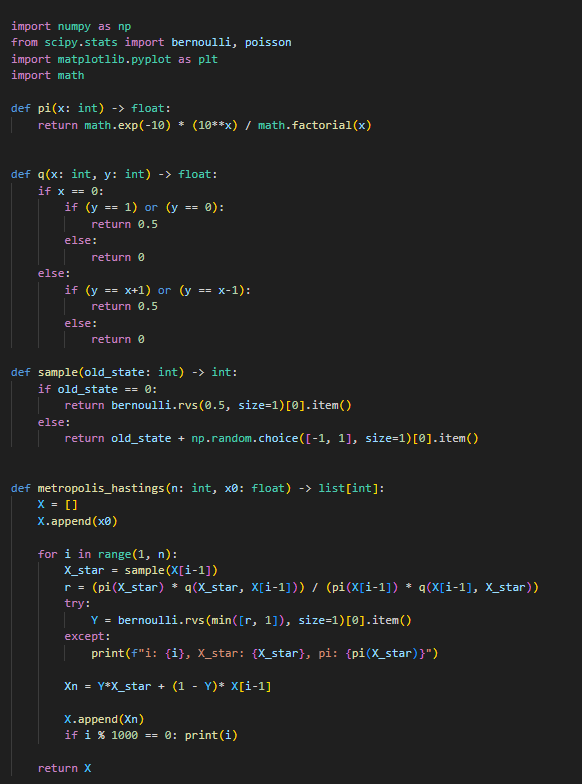
\includegraphics[width=\textwidth]{Images/Code 1.png}
    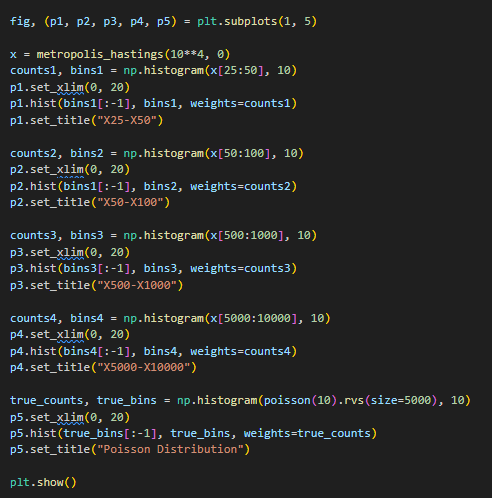
\includegraphics[width=\textwidth]{Images/Code 2.png}

    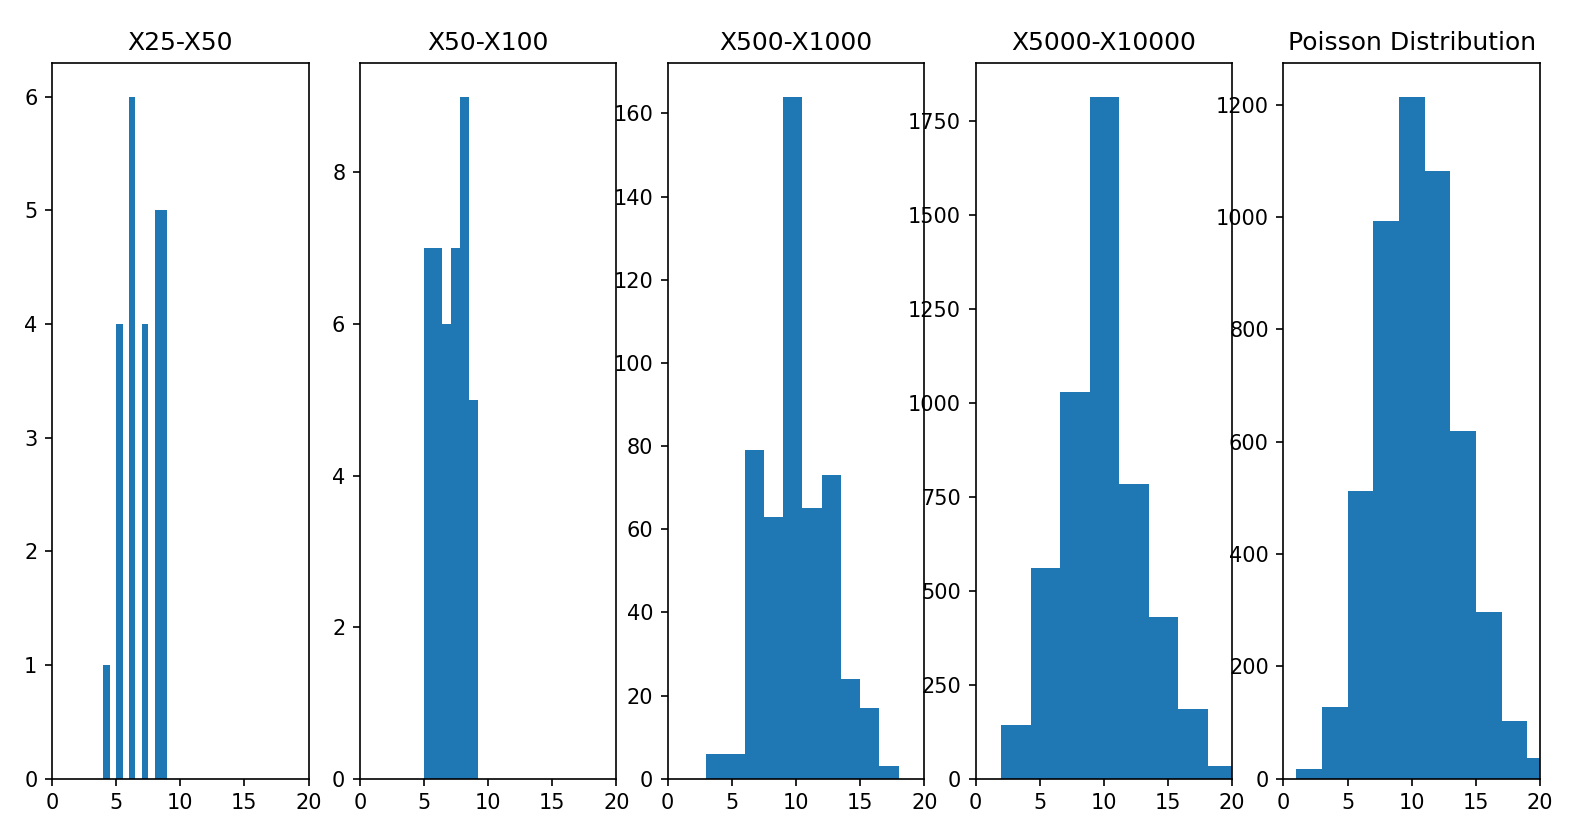
\includegraphics[width=\textwidth]{Images/Histograms.png}
\end{center}

\item (5 points) Suppose we have a 3-dimensional PMF $\pi(\xi_1,\xi_2,\xi_3)$, and it is strictly positive. Please provide a transition probability $p(\boldsymbol{x}, \boldsymbol{y})$ with $\boldsymbol{x}=(\xi_1,\xi_2,\xi_3)$ and $\boldsymbol{y}=(\eta_1,\eta_2,\eta_3)$ such that $\pi$ is the stationary distribution of $p$, i.e., $\pi$ and $p$ satisfy
\begin{align}\label{eq: 3D stationarity}
    \sum_{\xi_1}\sum_{\xi_2}\sum_{\xi_3} \pi(\xi_1,\xi_2,\xi_3) \cdot p\Big( (\xi_1,\xi_2,\xi_3), (\eta_1,\eta_2,\eta_3)\Big) = \pi(\eta_1,\eta_2,\eta_3),
\end{align}
which is equivalent to $\sum_{\boldsymbol{x}}\pi(\boldsymbol{x})p(\boldsymbol{x},\boldsymbol{y})=\pi(\boldsymbol{y})$. Specifically, please provide the formula of the $p(\boldsymbol{x},\boldsymbol{y})$ and prove Eq.~\eqref{eq: 3D stationarity}.

(There is more than one correct answer. You only need to provide one answer.)

Hint: The Gibbs sampling algorithm (Algorithm \ref{algorithm: Gibbs sampling}) with dimensionality $d=3$ is a hint. 

    \color{blue}
     
        Let $x = (\xi_1, \xi_2, \xi_3)^T$ and $y = (\eta_1, \eta_2, \eta_3)^T$ and then define
        \[\boxed{p(x, y) := \pi_{3\vert -3}(\xi_1, \xi_2, \eta_3) \cdot \pi_{2\vert -2}(\xi_1, \eta_2, \eta_3) \cdot \pi_{1\vert -1}(\eta_1, \eta_2, \eta_3)}\]  
        Where 
        \begin{align*}
            \pi_{3\vert -3}(\xi_1, \xi_2, \eta_3) &= \frac{\pi(\xi_1, \xi_2, \eta_3)}{\pi_{-3}(\xi_1, \xi_2)}\\
            \pi_{2\vert -2}(\xi_1, \eta_2, \eta_3) &= \frac{\pi(\xi_1, \eta_2, \eta_3)}{\pi_{-2}(\xi_1, \eta_3)}\\
            \pi_{1\vert -1}(\eta_1, \eta_2, \eta_3) &= \frac{\pi(\eta_1, \eta_2, \eta_3)}{\pi_{-1}(\eta_2, \eta_3)}
        \end{align*}
        So 
        \begin{align*}
            &\sum_{\xi_1} \sum_{\xi_2}\sum_{\xi_3} \pi(\xi_1,\xi_2,\xi_3) \cdot p\Big( (\xi_1,\xi_2,\xi_3), (\eta_1,\eta_2,\eta_3)\Big)\\
            &\qquad = \sum_{\xi_1}\sum_{\xi_2}\sum_{\xi_3} \pi(\xi_1,\xi_2,\xi_3) \cdot \pi_{3\vert -3}(\xi_1, \xi_2, \eta_3) \cdot \pi_{2\vert -2}(\xi_1, \eta_2, \eta_3) \cdot \pi_{1\vert -1}(\eta_1, \eta_2, \eta_3)\\
            &\qquad = \sum_{\xi_1}\sum_{\xi_2}\sum_{\xi_3} \pi(\xi_1,\xi_2,\xi_3) \cdot \frac{\pi(\xi_1, \xi_2, \eta_3)}{\pi_{-3}(\xi_1, \xi_2)} \cdot \frac{\pi(\xi_1, \eta_2, \eta_3)}{\pi_{-2}(\xi_1, \eta_3)} \cdot \frac{\pi(\eta_1, \eta_2, \eta_3)}{\pi_{-1}(\eta_2, \eta_3)}\\
            &\qquad = \sum_{\xi_1}\sum_{\xi_2} \pi_{-3}(\xi_1, \xi_2) \cdot \frac{\pi(\xi_1, \xi_2, \eta_3)}{\pi_{-3}(\xi_1, \xi_2)} \cdot \frac{\pi(\xi_1, \eta_2, \eta_3)}{\pi_{-2}(\xi_1, \eta_3)} \cdot \frac{\pi(\eta_1, \eta_2, \eta_3)}{\pi_{-1}(\eta_2, \eta_3)}\\
            &\qquad = \sum_{\xi_1}\sum_{\xi_2} \pi(\xi_1, \xi_2, \eta_3) \cdot \frac{\pi(\xi_1, \eta_2, \eta_3)}{\pi_{-2}(\xi_1, \eta_3)} \cdot \frac{\pi(\eta_1, \eta_2, \eta_3)}{\pi_{-1}(\eta_2, \eta_3)}\\
            &\qquad = \sum_{\xi_1} \pi_{-2}(\xi_1, \eta_3) \cdot \frac{\pi(\xi_1, \eta_2, \eta_3)}{\pi_{-2}(\xi_1, \eta_3)} \cdot \frac{\pi(\eta_1, \eta_2, \eta_3)}{\pi_{-1}(\eta_2, \eta_3)}\\
            &\qquad = \sum_{\xi_1}\pi(\xi_1, \eta_2, \eta_3) \cdot \frac{\pi(\eta_1, \eta_2, \eta_3)}{\pi_{-1}(\eta_2, \eta_3)}\\
            &\qquad = \pi_{-1}(\eta_2, \eta_3) \cdot \frac{\pi(\eta_1, \eta_2, \eta_3)}{\pi_{-1}(\eta_2, \eta_3)}\\
            &\qquad = \pi(\eta_1, \eta_2, \eta_3) \qed
        \end{align*}
    \color{black}

\end{enumerate}


%\bibliographystyle{plain}
\bibliography{sample}

\end{document}
